\documentclass{paper}
\usepackage{authblk}
\usepackage{float}
\usepackage[left=4cm, right=4cm]{geometry}

\usepackage{graphicx}
\graphicspath{{./img/}}

\title{Analyzing regression models for predicting the outcomes of Major League Baseball games}
\author[1]{Jeremy Moon}
\affil[1]{Institute for Computing in Research}
\date{August 2, 2024}

\begin{document}

\maketitle

\section{Introduction}
In a game of baseball, each team gets nine innings to score as many runs as they can. During each inning, batters face off in order against the opposing team's pitcher. The batter's objective: hit the ball, round the bases, and return to home plate---thus scoring a run. The pitcher's objective: prevent any of that from happening. The national pastime, as the sport became known, has been a part of American society for well over 100 years, producing numerous stars throughout its rich history. Cy Young, who won over 500 games as a pitcher; Babe Ruth, who hit more home runs alone than entire teams; Ted Williams, who remains the last man to hit .400 over a full season; Nolan Ryan, who struck out over 5,000 batters throughout his career. Historically, players were celebrated for their excellence in traditional stats---pitcher wins, home runs, batting average, and strikeouts.

As time passed, however, there was a shift. With advancements made in computing, more data were collected and analyzed. With more data available, new statistics were invented. It opened up new ways to evaluate a player's past performance. It opened up new ways to anticipate a player's future performance. And, by utilizing these advanced metrics, it opened up new ways to predict who was going to win the game.

This study aims to answer the question: What goes into predicting the outcomes of baseball games? The following sections will discuss the implementation of regression models, the analysis of results, and the exploration of potential improvements in an attempt to understand the inner workings of a prediction algorithm.

\subsection{Motivations}
There are several reasons why building a game prediction model might be useful in the context of baseball. Some of them are:

\begin{description}
\item[Analytical team building.] Being able to predict games---and seasons---in advance will provide insight into the strengths and weaknesses of the current team, which the front office can address by signing new players.
\item[Sports betting.] As the 1919 Black Sox scandal would suggest, sports betting has been around for quite some time. Using a trained model could be a more successful strategy for placing bets.
\item[Involved fan experience.] In addition to simply watching the games, fans can find predictions and later compare them to actual results. It'd be a more involved and interesting way for spectators to follow the action.
\item[In-depth study of statistics.] Personally, working on this project has been a huge opportunity to delve deeper into the statistics and learn about different tools available for implementing models with code.
\end{description}

\subsection{Setting a baseline}
The most rudimentary method for predicting the winner of each game---and for predicting anything, really---would be to randomly guess every outcome. While it certainly won't be very accurate, the random guessing model can provide a solid baseline to compare against when testing regression models. The random guessing model works as follows: for every game from the 2023 MLB season, one team will be predicted to score 1 run and the other team will be predicted to score 0 runs. The predictions will then be compared to actual results, evaluating whether the model correctly predicted the winning team.

\begin{figure}[H]
  \centering
  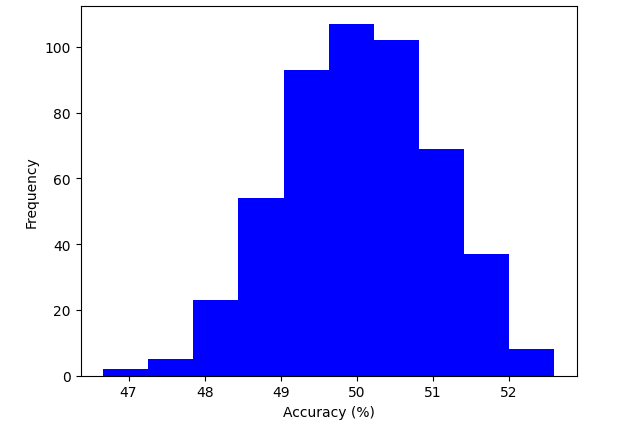
\includegraphics[width=8cm]{fig1}
  \caption{Distribution of accuracy for random guessing models.}
\end{figure}

This simulation process was run 500 times and produced the results as shown above. Unsurprisingly, the mean accuracy of the random guessing model was very close to 50\% and the standard deviation was right around 1\%. Assuming that the distribution of model accuracy is normal, it can be reasonably concluded that, 97.5\% of the time, the random guessing model will not exceed an accuracy of approximately 52\% (2 standard deviations higher than the mean). Therefore, the main objective of this study shall be to implement regression models that can consistently record an accuracy greater than 52\%.

\section{Data collection}
Before the model is created, data must first be collected. This section explains the data collection process.

\subsection{Selecting statistics}
The following statistics, collected for every regular season game from 2017 to 2023, were included in the dataset for training and testing:

\begin{itemize}
\item Team xwOBA differential
\item Lineup xwOBA
\item Team xFIP
\item Starting pitcher xFIP
\item Run differential
\item Win percentage in 1-run games
\end{itemize}

Each variable listed above will appear twice in the dataset, once for the home team and once for the away team.

Expected weighted on base average (xwOBA), provided by Baseball Savant, is the primary measure of offense. Weighted on base average (wOBA) describes how often a batter has reached base safely and how impactful he was in doing so. Hitting a home run would have more impact on the game than hitting a single (since a run is scored immediately with a home run but not always with a single), and wOBA rewards the batter accordingly. Expected wOBA, or xwOBA, is an estimate for what the batter's wOBA \textit{should've} been based on quality of contact, plate discipline, etc. This is likely a better indicator of future performance than plain wOBA because the element of luck is reduced.

Expected fielding independent pitching (xFIP), provided by FanGraphs, is the primary measure of defense. Fielding independent pitching (FIP) estimates how many runs a pitcher should expect to concede per 9 innings, based only on the three true outcomes (strikeouts, walks, and home runs---plays where the defense is not involved). Actual defense from the other 8 players is not considered for a couple of reasons: (1) defensive metrics generally have a weak correlation to team wins and (2) the majority of defensive plays are routine, meaning any player should be expected to make them.

Lastly, run differential (runs scored$-$runs allowed) measures the team's overall quality and win percentage in 1-run games measures the team's bullpen strength. Win percentage in 1-run games also indicates how ``clutch'' the team is, or how well they are able to come through in important moments late in the game.

\subsection{Assigning weights}
All of the aforementioned statistics were compiled using data from the last 3 years, including the current. In doing so, different weights were assigned to data from different years to ensure that the dataset contains the most accurate reflection of the current quality of teams and players.

First, stats were weighted based on season: 60\% for the current season, 25\% for the previous season, and 15\% for two seasons ago. Since many young players improve and many old players decline over the years, recent seasons will more closely reflect the player's current skill set.

Next, stats were also weighted based on sample size. The intuition is that a season in which the player was injured or in the minor leagues for a significant amount of time doesn't quite capture the player's abilities as much as a full healthy season. This step was only taken for individual stats, since team stats typically have similar sample sizes from year to year.

\subsection{Assumptions}
To simplify the real world baseball games, assumptions will have to be made. The regression models presented in this study assume the following:

\begin{description}
\item[Each game is independent of another.] This may be true; there are plenty of occurrences where a team gets blown out in one game, only to come back and win the next one. However, teams (and players) are susceptible to streaks, hot or cold.
\item[Environmental factors are irrelevant.] Weather, travel time, and amount of rest are variables that may or may not influence the outcome of any given game.
\item[All rookies have a rookie-average value.] Of course, not all rookies are created equal. Some rookies instantly become the next superstar, while many others struggle to adjust to the top level of competition.
\item[2020 was a normal year.] It was everything but. The pandemic-shortened 60-game season featured many impressive performances that likely would not have been sustained over the normal 162 games.
\end{description}

\section{Training the model}
With a dataset compiled, the model can begin to train. This section discusses the different types of regressions that were tested, and how each one can have its own benefits and drawbacks.

\subsection{Linear regression}
Linear regression takes the observed data and finds the linear relationship that best describes the trend shown. In a process called least squares regression, the model will attempt to minimize the sum of squared residuals. A residual can be defined as the vertical distance between the observed point and the fitted line, and can be either positive or negative. Summing the squared residuals, then, would reveal how much the observed data deviates from the fitted line. A linear regression model continually fits different lines until it finds the optimal slope, producing the following graph:

\begin{figure}[H]
  \centering
  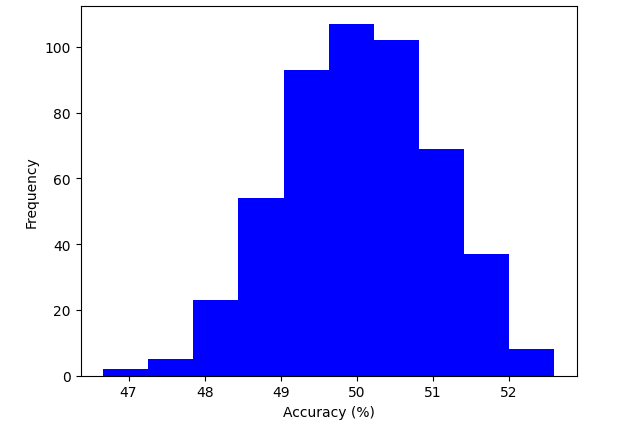
\includegraphics[width=1cm]{fig1}
  \caption{An example of linear regression. The fitted line has the equation $\hat{y}=\beta_0+\beta_1x_1$ where $\hat{y}$ is the response variable, $\beta_0$ is the y-intercept, $x_1$ is the explanatory variable, and $\beta_1$ is the coefficient for $x_1$ (in other words, the slope).}
\end{figure}

Using the fitted line, the value of $\hat{y}$ can easily be predicted for any value of $x_1$ (although the word "any" should be used with caution). If there are more explanatory variables, there would simply be more terms in the equation, as follows:

$$\hat{y}=\beta_0+\beta_1x_1+\beta_2x_2+\cdots+\beta_nx_n$$

In the context of this study, there are 12 explanatory variables, or features, used to predict the number of runs that a certain team will score. After preprocessing the input data to ensure they were all on the same scale, a linear regression model has been fitted using game data from 2017-2022 and tested using game data from 2023. The results, shown below, were fairly impressive for such a simple model.

\begin{figure}[H]
  \centering
  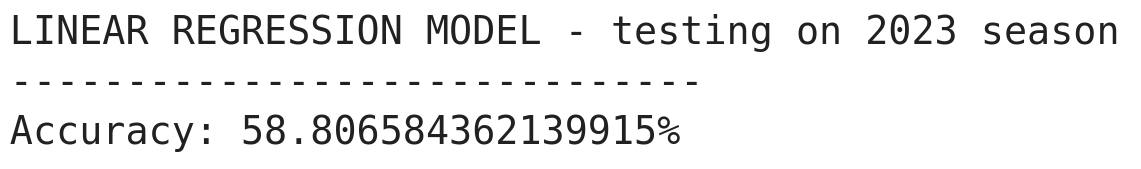
\includegraphics[width=8cm]{fig2}
  \caption{Results from linear regression model.}
\end{figure}

An accuracy of 58.27\% certainly exceeds the aforementioned goal of 52\%. Furthermore, it comes very close to the accuracy achieved by Vegas betting odds ([??]\%). In fact, when the model was fitted using game data from 2017-2018, 2020-2023 and tested using game data from 2019, it had an even better accuracy of 61.10\%.

Despite the accuracy, though, there is reason to look at this linear regression model with a little bit of skepticism. With most linear regressions, when using an $x$-value beyond the range for which the fitted line was generated, the predicted $y$-value can often be unrealistic or uninterpretable. For instance, when the model was given a scenario where a very good team plays against a very bad team, it predicted that the latter will score negative runs.

\begin{figure}[H]
  \centering
  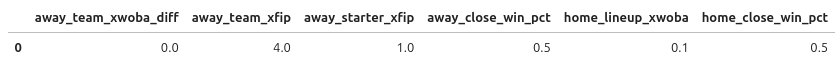
\includegraphics[width=13cm]{fig3}
  \caption{Input values for linear regression. Notably, the away team starting pitcher's xFIP is a stellar 1.00, while the home team lineup's xwOBA is a beyond-terrible .100.}
  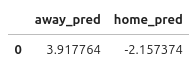
\includegraphics[width=4cm]{fig4}
  \caption{Output values for linear regression. The home team is expected to score an unrealistic -2.16 runs.}
\end{figure}

Granted, it is extremely unlikely that anyone will carry a 1.00 xFIP or .100 xwOBA over 3 seasons, but it may still be worth looking beyond the accuracy and considering these issues when evaluating the overall quality of the prediction model.

\subsection{Poisson regression}
When trying to predict how many events will occur over a given time interval, the Poisson regression becomes a useful tool. It certainly fits the purpose of this study, which is to predict how many runs a team will score in 9 innings. Unlike linear regression, the observed data will be fitted to an exponential curve, yielding the following equation:

$$\log(\lambda)=\beta_0+\beta_1x_1+\beta_2x_2+\cdots+\beta_nx_n$$

where $x$ represents each explanatory variable, $\beta$ represents their coefficients, and $\lambda$ represents the mean number of occurrences. To predict the value of the response variable, a random selection is made following the Poisson distribution with the given $\lambda$. The Poisson distribution, as shown below, is a discrete distribution that indicates the probability of observing a certain number of occurrences.

\begin{figure}[H]
  \centering
  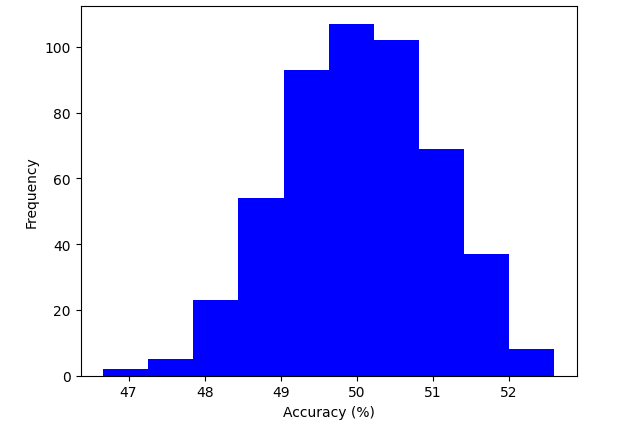
\includegraphics[width=1cm]{fig1}
  \caption{An example of Poisson distribution.}
\end{figure}

One interesting property of the Poisson distribution is that mean equals variance (which equals lambda). Consider this: the average points per team scored in an NBA game during the 2023-24 season was 114.2. Typically, NBA teams will score anywhere from 80 to 130 points in any given game. In contrast, the average goals per team scored in a Premier League match during the 2023-24 season was much lower at 1.64, and teams will usually score no more than 5 goals on a good day. The intuition is that if the count being predicted is large, then possible values will have a wider range, and vice versa.

\begin{figure}[H]
  \centering
  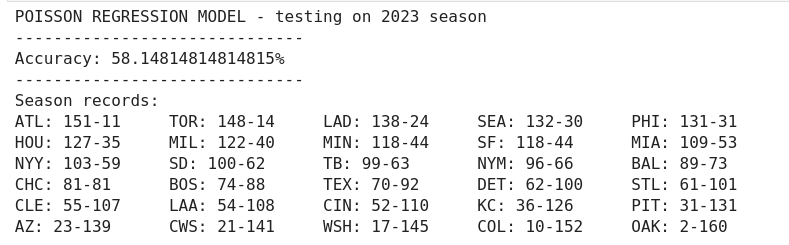
\includegraphics[width=13cm]{fig5}
  \caption{Results from Poisson regression model.}
\end{figure}

After preprocessing the input data to ensure they were all on the same scale, a Poisson regression model has been fitted using game data from 2017-2022 and tested using game data from 2023. The results were fairly comparable to linear regression in terms of accuracy, with the added benefit of never predicting negative run totals. Another issue appears, however, when the aggregate is examined. After traversing through all the prediction for 2023, a season record for each team was calculated---records that were, compared to real life, very extreme. The Atlanta Braves (ATL) are certainly World Series contenders, but they aren't an unprecedented powerhouse. The Oakland Athletics (OAK) are sitting bottom of the American League West, but they certainly win more than 2 games in a full season. In fact, this problem also appeared when testing the linear regression model. The statistically better team was being favored a little too much, resulting in bias.

Tuning the ``alpha'' parameter may yield more realistic results in terms of season record. Sure enough, with alpha set to 9, the Braves come back down to earth and the Athletics can avoid losing their entire fanbase. This improvement did come at a cost, namely about 4\% of accuracy. While the model remains comfortably above the goal of 52\%, it demonstrates the trade-off that occurs between individual game accuracy and realistic aggregate results. Selecting the right model and the right parameters, therefore, should depend on the user's purpose in making predictions. After all, no one model will be optimized to be the best in every aspect.

\begin{figure}[H]
  \centering
  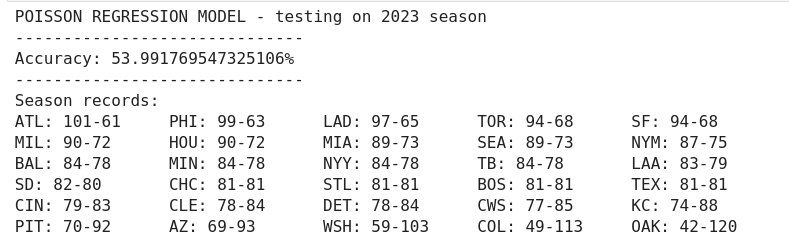
\includegraphics[width=13cm]{fig6}
  \caption{Results from Poisson regression model after adjusting the ``alpha'' parameter. While the accuracy dropped to 53.99\%, season records became much more realistic.}
\end{figure}

\subsection{Random forest regression}
Choosing what (and where) to eat for lunch is a decision made after taking into account several factors, such as cost, distance, and reviews. When deciding if a certain restaurant will be a good choice, one might consider if it costs less than \$15, is located within 1 mile, and is rated above 4 stars. This decision-making process can be modeled using a decision tree, visualized below. Starting at the top of the tree, called the root node, an expression is evaluated to be either true or false. If true, the path labeled "true"---or the path to the left, in the case where paths are unlabeled---is followed and the previous step is repeated with a different expression. If false, the same thing happens except that the other path (typically to the right) is followed. These steps are repeated until a leaf node---a node with no paths emerging out of it---is reached and a conclusion is made.

\begin{figure}[H]
  \centering
  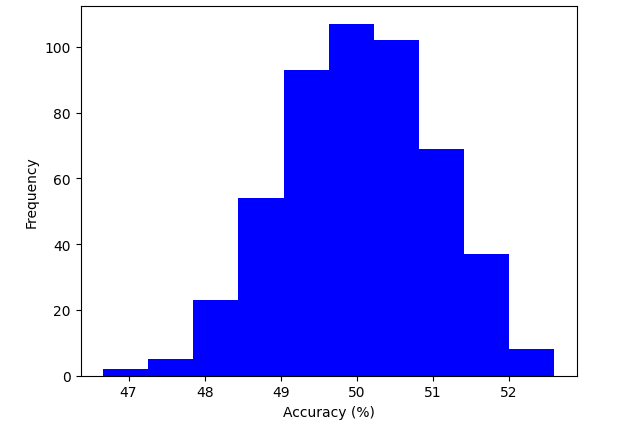
\includegraphics[width=1cm]{fig1}
  \caption{An example decision tree.}
\end{figure}

A similar model can be constructed with an observed dataset. The process of building a decision tree starts with generating an expression to be evaluated at the root node, and data points are separated into two groups based on that expression. Next, the algorithm will repeatedly test whether using a different expression---whether that's evaluating a different variable or comparing against a different value---will result in a more effective split. The goal is to achieve the lowest impurity at every step, to ensure that each split results in the most similar data points grouped together. Gini index, entropy, and information gain are some of the most common metrics for numerically representing impurity.

A random forest is simply a collection of multiple decision trees. Rather than having one tree make the decision all by itself, many differently-constructed trees each compute an output, with the final decision being either the most common output or the average of all outputs. As a result, a random forest tends to have a lower likelihood of overfitting than a decision tree. When a model is overfitted, it becomes too dependent on training data; it performs very well when given the same training data but not so well with any other dataset. In the realm of predictions, this is bad news because there is no guarantee that future inputs will be exactly the same as past inputs.

\begin{figure}[H]
  \centering
  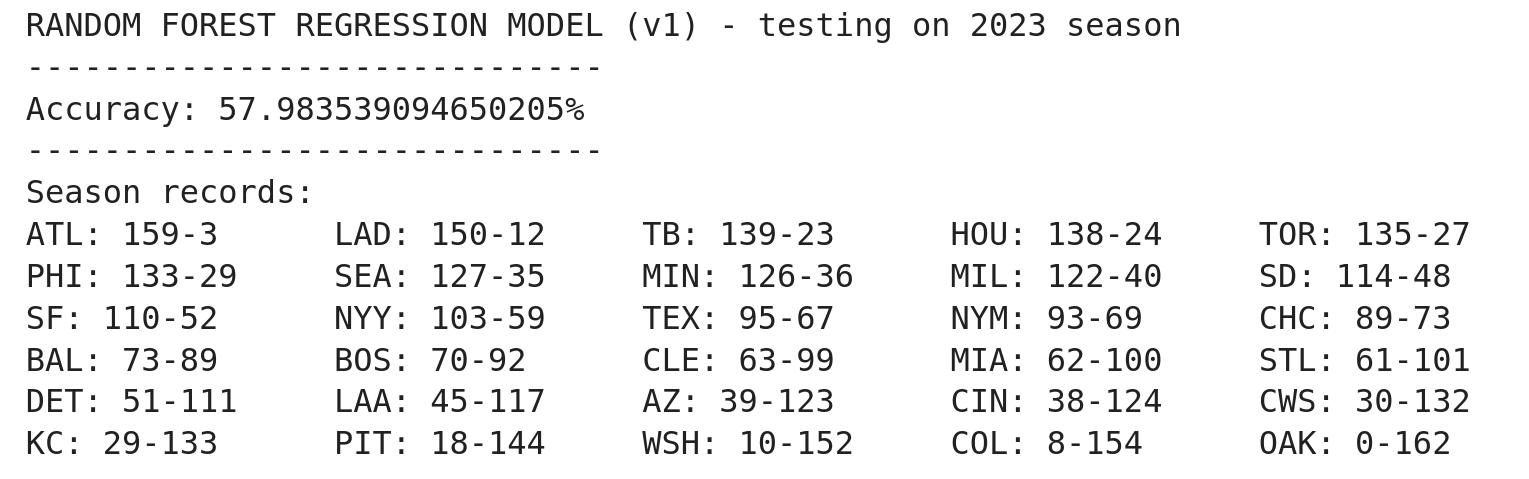
\includegraphics[width=13cm]{fig7}
  \caption{Results from random forest regression model.}
\end{figure}

As with all other models, a random forest regressor has been fitted using game data from 2017-2022 and tested using game data from 2023. Initially, the regressor consisted of 500 decision trees, and produced a result similar to the other two models: accuracy around 58\%, with skewed season record numbers. Reducing the number of decision trees to only 5 yielded a more reasonable season record at the cost of about 5\% of accuracy.

\begin{figure}[H]
  \centering
  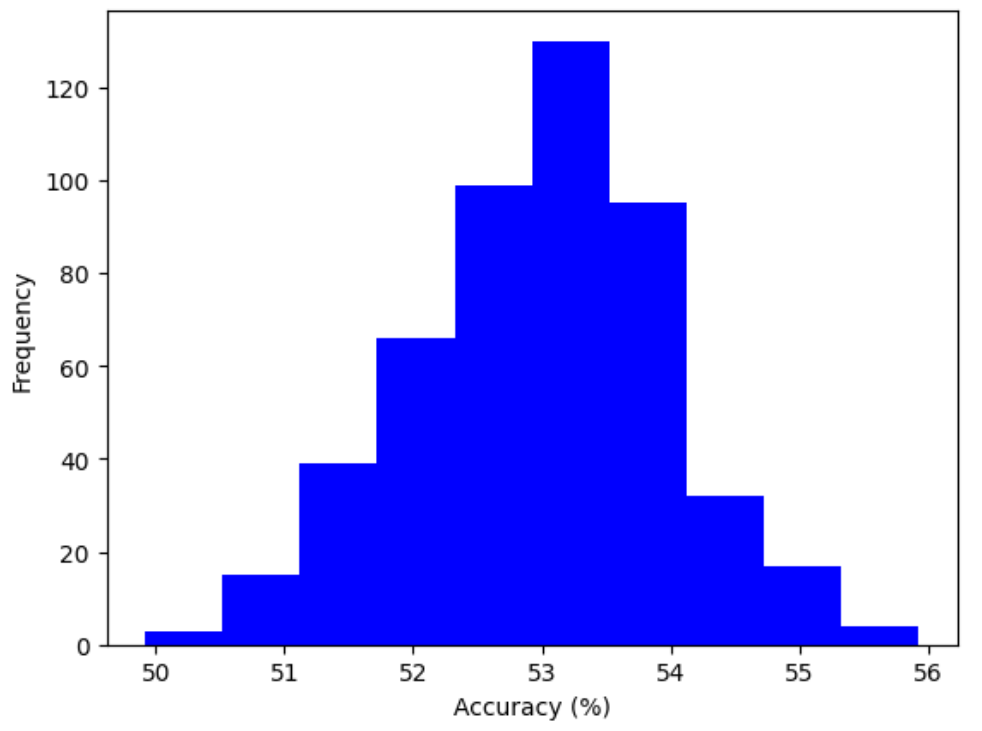
\includegraphics[width=8cm]{fig8}
  \caption{Distribution of accuracy for random forest regression models with 5 decision trees. While the mean is still over the goal, there are a handful of data points below the 52\% threshold.}
\end{figure}

So how exactly did this random forest regressor work? In particular, what features were being used to make the decision? The figure below visualizes part of one individual decision tree for predicting how many runs the home team will score.

\begin{figure}[H]
  \centering
  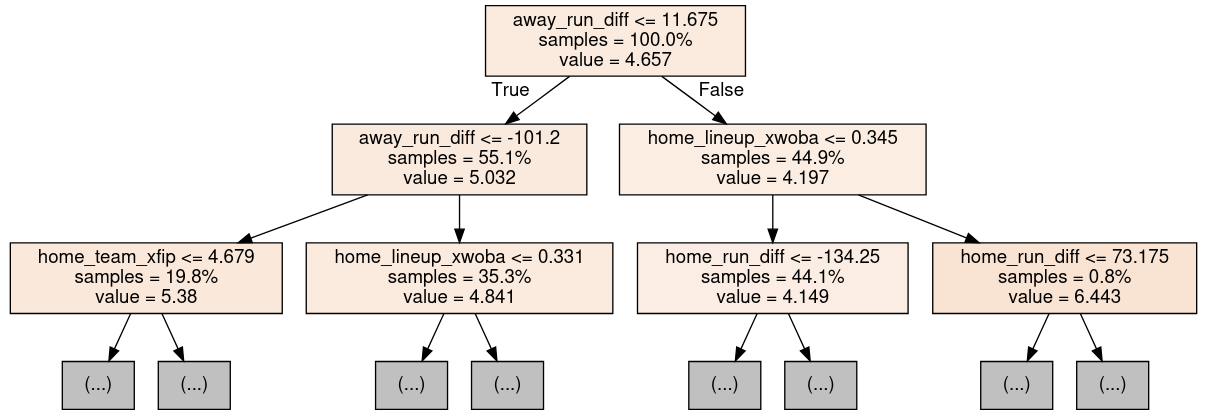
\includegraphics[width=13cm]{fig9}
  \caption{A sample decision tree within the random forest regression model.}
\end{figure}

The bottom left node evaluates the home team's xFIP which, from a logical standpoint, is quite odd. The home team's \textit{pitching} shouldn't affect the home team's \textit{batting}, yet the decision tree implies so. In fact, the random forest model weighed the home team's xFIP at about 6\% and, more surprisingly, the home team starting pitcher's xFIP at about 12\%. It is reasonable to believe that the home team starter's xFIP shouldn't be the third most important factor when predicting the home team's runs scored.

\begin{figure}[H]
  \centering
  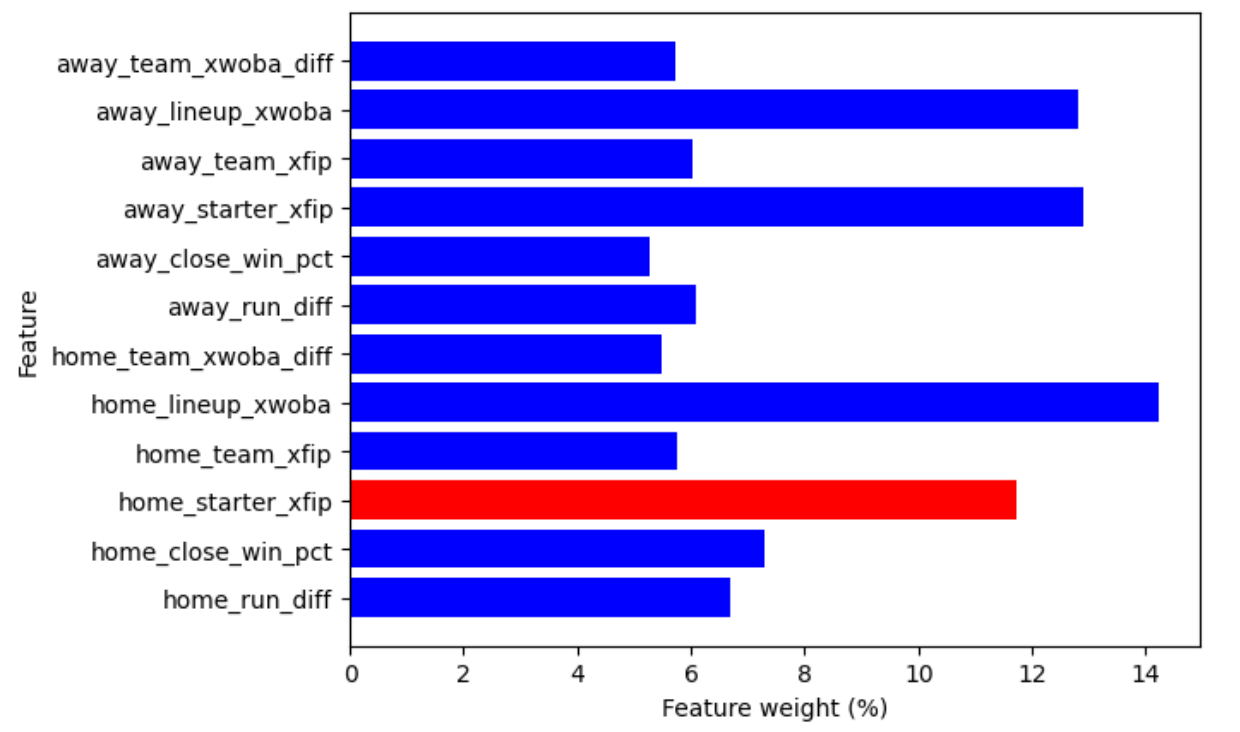
\includegraphics[width=11cm]{fig10}
  \caption{Feature weights for random forest regression model.}
\end{figure}

The random forest regression model was run again, this time without irrelevant features---that left 8 features. While there was no significant change in the results, it was worth ensuring that the model isn't making any misled decisions. The features used for this modified random forest regression model is shown below, along with their feature importance values.

\begin{figure}[H]
  \centering
  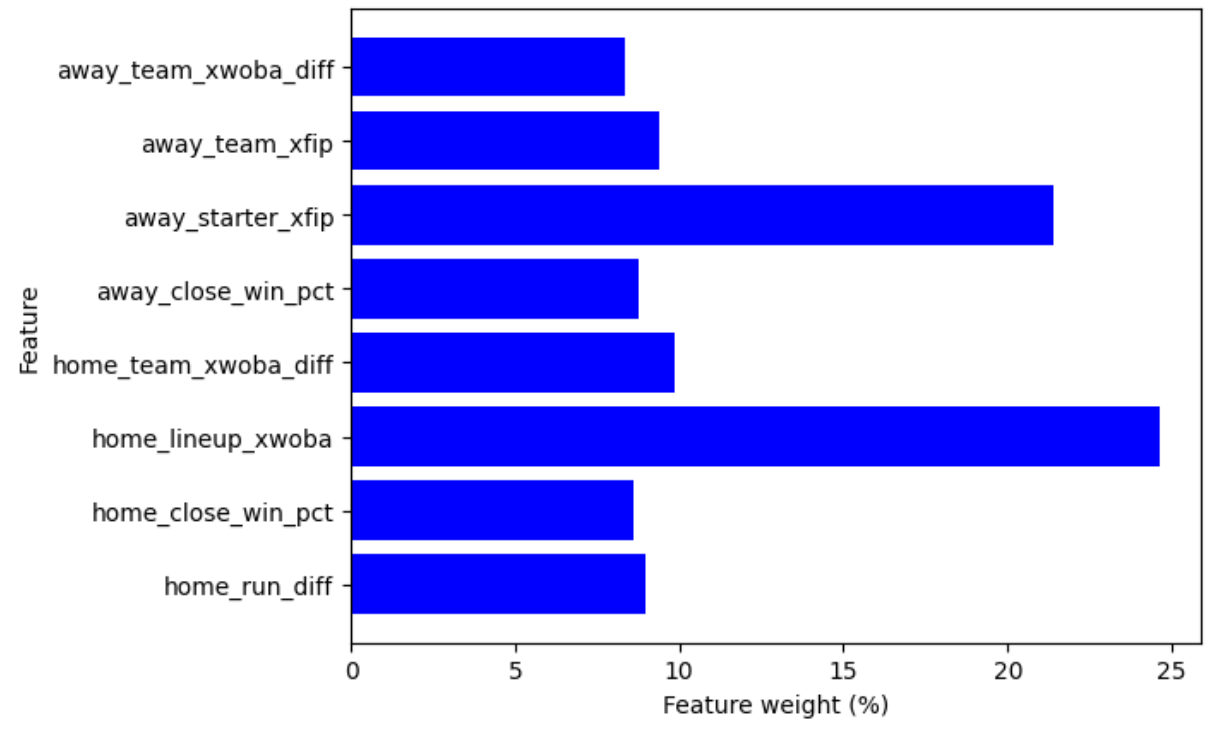
\includegraphics[width=11cm]{fig11}
  \caption{Feature weights for random forest regression model after removing irrelevant features.}
\end{figure}

Now, the home team's lineup and the away team's starting pitcher have the biggest influence in predicting the home team's score---just as expected. Overall, the random forest regression model features more variability due to randomness, but it more closely resembles the human decision making process than the other two regressions.

\section{Discussion}
This study demonstrated that, using various measures of offense, defense, and overall team quality, it was possible to predict the outcomes of MLB games. Most of the models discussed stayed comfortably above the 52\% goal established in the beginning. The models have a variety of potential uses, mentioned previously in the Motivations section, but there are also key takeaways and points of caution that will be explored in this section.

\subsection{Limitations}
Statcast, and by extension xwOBA, came out in 2015, meaning there are only 10 years' worth of data to work with. While it seems unlikely that using a larger dataset would increase accuracy, it could increase stability and reduce variability. This is especially true regarding to issue of extrapolation; having more data would allow models to encounter more potential scenarios and generate more reasonable predictions for rare cases.

Additionally, all models included in this paper made assumptions as listed previously, yet not all assumptions would turn out to be true in the real world. Attempting to take into account all of the factors would involve huge amounts of data that is beyond the scope of this study.

\subsection{Key takeaways}
\begin{description}
\item[Look beyond the surface level results.] Taking a look beyond the surface level result, namely accuracy, provided some surprising insight into potential bias and skewness.
\item[Complexity doesn't always yield the best outcomes.] Linear regression, mathematically the simplest model of the three, yielded the best accuracy. Some features were even discarded to prevent irrelevant variables from adding noise. There is no need to add unnecessary complexity into any program without proof that it will enhance its performance.
\item[Identify and balance trade-offs.] The results of this study featured a trade-off between accuracy and realistic aggregate records. Balancing the two depends on the overall purpose of using the model, whether that's placing bets (where accuracy would be preferred) or identifying the team's weaknesses (where realistic results would be preferred).
\end{description}

\section{Acknowledgments}

\section{Works Cited}

\end{document}
